\documentclass{standalone}
\usepackage{tikz}
\usepackage{ctex,siunitx,ninecolors}
\setCJKmainfont{Noto Serif CJK SC}
\usepackage{tkz-euclide}
\usepackage{amsmath}
\usepackage{wasysym}
\usetikzlibrary{patterns, calc}
\usetikzlibrary{decorations.pathmorphing, decorations.pathreplacing, decorations.shapes,3d}
\pgfdeclareverticalshading{pile}{100bp}{
  color(0bp)=(black);color(40bp)=(black);color(50bp)=(white);color(60bp)=(black);color(100bp)=(black)
}
\pgfdeclareverticalshading{pile2}{100bp}{
  color(0bp)=(white);color(50bp)=(black);color(100bp)=(white)
}
\begin{document}
\small
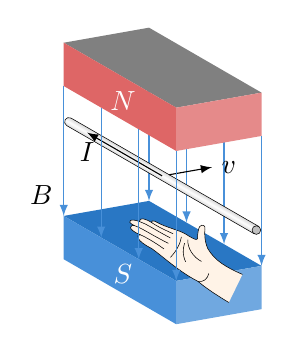
\begin{tikzpicture}[>=latex,scale=1.1]
  \useasboundingbox(0.1,-0.75)rectangle(-2.7,2.75);
  \begin{scope}[xscale=-1]
    \fill[azure5](0,0)--(30:1.5)--++(-10:1.0)--++(-150:1.5)--cycle;
    \fill[azure6](-10:1.0)--++(30:1.5)--++(0,-0.5)--++(-150:1.5)--cycle;
    \fill[azure7](0,0)--(-10:1.0)--++(0,-0.5)--++(170:1.0)--cycle;
    \foreach \x in {0,0.5,1,1.5}
    {
      \draw[azure6,<-](30:\x)--++(0,1.5);
    }
    \fill[gray](0,2)--++(30:1.5)--++(-10:1.0)--++(-150:1.5)--cycle;
    \fill[red6]([yshift=2cm]-10:1.0)--++(30:1.5)--++(0,-0.5)--++(-150:1.5)--cycle;
    \fill[red7](0,2)--++(-10:1.0)--++(0,-0.5)--++(170:1.0)--cycle;
    \node at (1.6,1.9)[text=white]{$N$};
    \node at (1.6,-0.1)[text=white]{$S$};
    \node at (2.3,0.6)[above left]{$B$};
    \draw[shading=pile,shading angle=150,very thin](0.034,0.456)--(2.199,1.706)arc(120:-60:0.05)--(0.084,0.370)--cycle;
    \draw[fill=lightgray,very thin](0.0594,0.4132)circle(0.05);
    \draw[->](1.065,1.052)--++(170:0.5)node[right]{$v$};
    \draw[->](1.148,1.039)--++(30:1.0)node[below]{$I$};
    \fill[pink!10!orange!10,draw=black,very thin](0.220,-0.099)..controls(0.412,-0.014)and(0.538, 0.058)..
    (0.621, 0.200)..controls(0.657, 0.283)and(0.661, 0.376)..
    (0.653, 0.425)..controls(0.646, 0.464)and(0.680, 0.487)..
    (0.714, 0.454)..controls(0.727, 0.436)and(0.739, 0.376)..
    (0.739, 0.317)..controls(0.741, 0.295)and(0.768, 0.298)..
    (0.868, 0.362)..controls(0.958, 0.419)and(1.084, 0.433)..
    (1.235, 0.516)..controls(1.265, 0.529)and(1.270, 0.516)..
    (1.268, 0.500)..controls(1.341, 0.544)and(1.407, 0.566)..
    (1.411, 0.512)..controls(1.493, 0.546)and(1.582, 0.526)..
    (1.473, 0.467)..controls(1.504, 0.474)and(1.570, 0.433)..
    (1.403, 0.360)..controls(1.453, 0.359)and(1.442, 0.286)..
    (1.274, 0.204)..controls(1.165, 0.130)and(0.958,-0.065)..
    (0.736,-0.178)..controls(0.690,-0.213)and(0.638,-0.265)..(0.378,-0.423);
    \draw[very thin](0.736,-0.178)..controls(0.672,-0.196)and(0.620,-0.146)..(0.609,-0.088)
    (0.693,0.051)..controls(0.787,0.098)and(0.858,0.205)..(0.851,0.304)
    (0.889,0.262)..controls(0.909,0.190)and(0.914,0.129)..(0.876,0.046)
    (0.925,0.335)..controls(0.938,0.252)and(0.985,0.168)..(1.052,0.098)
    (1.021,0.371)..controls(1.110,0.411)and(1.209,0.458)..(1.268,0.500)
    (1.053,0.323)..controls(1.237,0.419)and(1.313,0.478)..(1.411,0.512)
    (1.076,0.260)..controls(1.300,0.374)and(1.375,0.433)..(1.473,0.467)
    (1.127,0.196)..controls(1.244,0.280)and(1.346,0.337)..(1.403,0.360);
    \foreach \x in {0,0.5,1,1.5}
    {
      \draw[azure6,<-]([shift=(-10:1.0)]30:\x)--++(0,1.5);
    }
  \end{scope}
\end{tikzpicture}
\end{document}